\documentclass[11pt]{article}

\usepackage[letterpaper,margin=0.75in]{geometry}
\usepackage{booktabs}
\usepackage{graphicx}
\usepackage{listings}

\setlength{\parindent}{1.4em}

\begin{document}

\lstset{
  language=Python,
  basicstyle=\small,          % print whole listing small
  keywordstyle=\bfseries,
  identifierstyle=,           % nothing happens
  commentstyle=,              % white comments
  stringstyle=\ttfamily,      % typewriter type for strings
  showstringspaces=false,     % no special string spaces
  numbers=left,
  numberstyle=\tiny,
  numbersep=5pt,
  frame=tb,
}

\title{Lab 1 Report: Network Simulation}

\author{Kevin DeVocht}

\date{}

\maketitle

\section{Two Nodes}
For the first simulation, the packet was created at 0 seconds, with an identifier of 1 and it was recieved at 1.08 seconds.
For the second simulation, the packe was created at 0 seconds, with an identifier of 1 and it was recieved at 80.01 seconds.
For the last simulation of this section, the first, second and third packets were all created at 0 seconds, while the fourth one was created at 2 seconds.
The identifiers for the first, second, third and fourth packets are 1, 2, 3 and 4 respectively.
The first packet arrived at 0.018 seconds.  The second packet arrived at 0.026 seconds.  The third packet arrived at 0.034 seconds and finally. the fourth packet arrived at 2.018 seconds.


\vspace{0.5cm}
\begin{tabular}{|l|l|l|l|} \hline
Simulation & Creation Time & Identity & Arrival Time\\
\midrule
1 & 0 & 1 & 1.08\\
2 & 0 & 1 & 80.01\\
3 & 0 & 1 & 0.018\\
3 & 0 & 2 & 0.026\\
3 & 0 & 3 & 0.034\\
3 & 2 & 4 & 2.018\\
\bottomrule
\end{tabular}
\vspace{0.5cm}

For part all three parts we used a network with just two nodes n1 and n2.  We created a connection from n1 to n2 and another connection from n2 back to n1.  For the first section we set the bandwidth of both connections at
1 Mbps.  We also set the propagation delay at 10 ms for both connections.  For the second section's network we changed the bandwidth to 100bps on both connections

\section{Three Nodes}

\section{Queuing Theory}

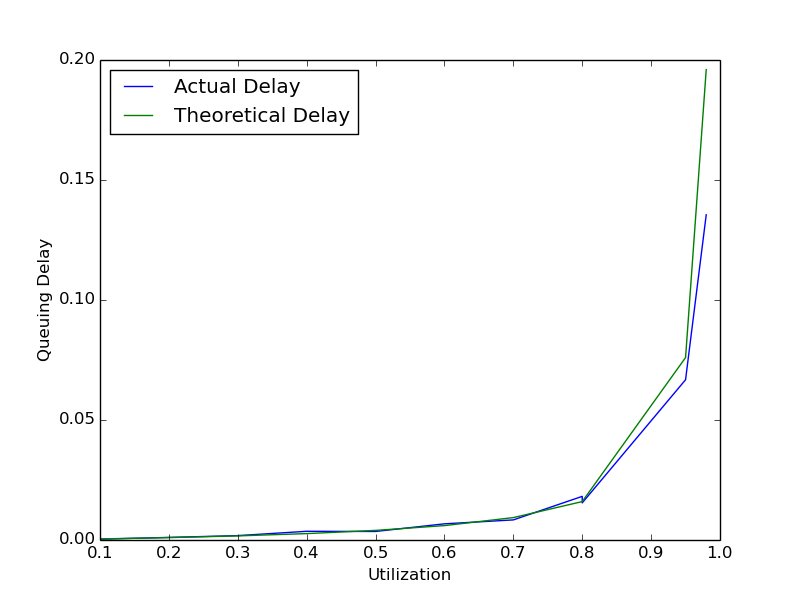
\includegraphics[width=11cm]{test.png}

\end{document}